\documentclass[conference]{IEEEtran}

% Core typography and layout packages
\usepackage[utf8]{inputenc}
\usepackage[T1]{fontenc}
\usepackage{microtype}
\usepackage{url}
\usepackage{cite}

% Mathematical packages
\usepackage{amsmath}
\usepackage{amssymb}
\usepackage{amsfonts}

% Table packages
\usepackage{booktabs}
\usepackage{multirow}
\usepackage{array}

% Graphics and Plotting packages
\usepackage{graphicx}
\usepackage{xcolor}
\usepackage{tikz}
\usetikzlibrary{shapes.geometric, arrows, positioning, fit, calc}
\usepackage{pgfplots}
\pgfplotsset{compat=1.18}

% Hyperref (configured to avoid IEEEtran clash)
\usepackage{hyperref}
\hypersetup{
    colorlinks=true,
    linkcolor=black,
    citecolor=black,
    urlcolor=black
}

% Title and Metadata
\title{ManiGit: Transparent, Versioned Context Memory\\for Long-Running AI Agents}

\author{
    \IEEEauthorblockN{Arshmeet Singh}
    \IEEEauthorblockA{\textit{Chandigarh University} \\
    Mohali, Punjab, India}
}

\begin{document}

\maketitle

\begin{abstract}
As autonomous AI agents are deployed for multi-session and long-horizon tasks, managing accumulated conversational context becomes a primary failure point. Standard memory architectures rely either on uncurated in-context prompt stuffing, lossy running summaries, or vector databases that execute destructive in-place mutations. Consequently, existing systems suffer from context budget exhaustion, lack historical auditability, and introduce catastrophic ``ghost context'' when new facts contradict prior instructions. In this paper, we propose \textbf{ManiGit}, an open architecture providing transparent, versioned context memory for long-running agents. ManiGit decouples persistent memory accumulation from bounded prompt assembly by combining: (1) an immutable SQLite message archive with commit-linked explicit provenance; (2) a Directed Acyclic Graph (DAG) commit substrate tracking active memory states; (3) a four-tier memory lifecycle state machine (\texttt{VERBATIM}, \texttt{SUMMARY}, \texttt{ARCHIVED}, \texttt{TOMBSTONE}); (4) automated contradiction supersession accompanied by auditable Why Reports; and (5) a deterministic greedy knapsack context compiler that enforces strict adherence to arbitrary token budgets $B$. 

Across 880 controlled experimental trials evaluating 8 methods/variants across 11 multi-turn scenarios and 5 token budgets ($B \in [128, 2048]$), ManiGit achieves 86.4\% factual recall [95\% CI: 78.7\%, 91.6\%] and 86.4\% answer correctness while consuming 43.0\% fewer context tokens than Full History, maintaining 100\% compliance with token budgets. Furthermore, in our evaluated benchmark scenarios, ManiGit delivers 100\% accuracy on point-in-time historical reconstruction queries where baseline RAG and sliding windows score 0\%. Controlled ablations quantitatively isolate the individual contributions of contradiction supersession (-5.0\% degradation when ablated), confidence calibration (-5.0\% degradation), and tier-aware ranking (preventing a 100\% loss of verbatim constraints under tight budgets of $B=128$). The evaluation pipeline, experiment configurations, and raw benchmark artifacts are organized to support reproducibility.
\end{abstract}

\begin{IEEEkeywords}
Large Language Models, LLM Agents, Agent Memory, Persistent Memory, Context Management, Versioned Memory, Token-Budget Optimization.
\end{IEEEkeywords}

% Modular Sections
\section{Introduction}
\label{sec:introduction}

Autonomous agents powered by Large Language Models (LLMs) are increasingly deployed to execute multi-turn, long-horizon tasks, including software development~\cite{wu2025gcc}, multi-session customer support~\cite{deshmukh2024mem0}, scientific exploration, and interactive simulations~\cite{park2023generative}. As these agents interact with users and external environments over days or weeks, they accumulate extensive conversational histories, tool executions, and evolving operational constraints. Managing this accumulated state poses a fundamental challenge: while the agent must retain knowledge of foundational decisions made in early sessions, it must also adapt when those decisions are superseded by newer instructions, all while remaining strictly bounded by finite context budgets~\cite{packer2023memgpt,liu2024lost}.

Historically, agent state management has relied on a continuum of heuristic approximations. Simple \textit{sliding windows} preserve immediate conversational flow but suffer catastrophic forgetting of early project constraints. \textit{Running summarization} compresses conversational history into natural language preambles, but inevitably suffers from information flattening, semantic drift, and irreversible loss of exact technical specifications. \textit{Retrieval-Augmented Generation} (RAG)~\cite{lewis2020retrieval,guu2020realm} and vector-based memory layers~\cite{deshmukh2024mem0} index historical snippets into dense embedding spaces; however, standard retrieval models treat all chunks as timeless truths. When a user changes an instruction (e.g., migrating from PostgreSQL to MongoDB), vector similarity search frequently retrieves both the outdated initial configuration and the updated requirement, introducing conflicting ``ghost context'' that degrades model reasoning~\cite{stale2025benchmark,wu2024longmemeval}.

Recent architectural advances have significantly expanded the nominal context windows of modern foundation models, extending capacity from 4,096 tokens to 128k, 1M, and 2M tokens~\cite{brown2020language,dong2023bamboo}. However, empirical research demonstrates that larger context windows do not solve the memory challenge~\cite{liu2024lost,maharana2024locomo}. First, stuffing massive histories into prompts incurs severe linear or quadratic inference latency and high financial costs. Second, frontier models exhibit the ``Lost-in-the-Middle'' phenomenon, where factual recall deteriorates when critical information is placed in the center of long contexts~\cite{liu2024lost}. Third, in-context prompt stuffing provides no persistence across independent inference calls and offers zero mechanisms for historical auditing or branch exploration. In short, \textbf{large context capacity does not eliminate the necessity for principled context curation}.

Most critically, existing persistent memory architectures commonly employ \textit{destructive update mechanics}~\cite{packer2023memgpt,deshmukh2024mem0,zhou2025ltmsecurity}. When new facts arrive, frameworks typically execute in-place text replacements or database \texttt{UPDATE} operations, permanently erasing previous configurations. When an agent produces an unexpected output or hallucinates, human auditors have no mechanism to reconstruct what the agent believed at that specific point in time. Destructive updates also render agents incapable of answering retrospective historical queries (e.g., ``What was our database target before Tuesday's meeting?'') after factual supersession has occurred.

To address these compounding limitations, we propose \textbf{ManiGit}, an open architecture providing transparent, versioned context memory for long-running AI agents. ManiGit decouples persistent memory accumulation from bounded prompt context assembly by integrating:
\begin{enumerate}
    \item \textbf{An Immutable Message Archive:} An append-only SQLite repository that permanently preserves raw conversation turns with content hashing and session provenance.
    \item \textbf{A Directed Acyclic Graph (DAG) Commit Substrate:} A Git-inspired commit tree where each factual state change is recorded as an immutable, parent-linked commit object, enabling complete auditability and non-destructive historical checkout.
    \item \textbf{Hybrid Rule-First and Confidence-Calibrated Memory Intake:} An intake pipeline that routes unambiguous technical constraints through zero-latency pattern rules, while passing ambiguous candidate assertions to an LLM judge calibrated with explicit confidence thresholds.
    \item \textbf{A Four-Tier Memory Lifecycle Model:} Classifying facts into functional lifecycle states (\texttt{VERBATIM}, \texttt{SUMMARY}, \texttt{ARCHIVED}, \texttt{TOMBSTONE}), isolating superseded or refuted facts from active prompt compilation while retaining them for historical reconstruction.
    \item \textbf{Automated Contradiction Supersession and Why Reports:} Automatically detecting when a new fact contradicts an active fact, archiving the superseded fact, and generating an auditable Why Report recording the classification rule, confidence score, and supersession target.
    \item \textbf{Token-Budget Context Compilation:} Formulating prompt context assembly as a constrained knapsack problem, solved via a greedy score-density compiler that enforces strict compliance with arbitrary token budgets $B$.
\end{enumerate}

Through a rigorous controlled evaluation comprising 880 experimental trials across 11 scenarios, 8 methods/variants, and 5 token budgets ($B \in [128, 2048]$), we demonstrate that ManiGit achieves 86.4\% fact recall [95\% CI: 78.7\%, 91.6\%] while consuming 43.0\% fewer context tokens than Full History and consistently maintaining 100\% compliance with token budgets. Furthermore, in our evaluated benchmark scenarios, ManiGit achieves 100\% accuracy on point-in-time historical reconstruction queries where baseline RAG and sliding windows score 0\%. Controlled ablations quantitatively isolate the contribution of contradiction supersession (-5.0\% degradation when removed), confidence thresholding (-5.0\% degradation when removed), and tier-aware ranking (-1.0\% overall degradation, dropping to 0\% recall on targeted tier competition at $B=128$). The evaluation pipeline, experiment configurations, and raw benchmark artifacts are organized to support reproducibility.

\section{Background}
\label{sec:background}

To contextualize ManiGit's architectural contributions, we review the foundational concepts governing context dynamics, retrieval augmentation, and agent memory management.

\subsection{Long-Context Language Models}
The Transformer architecture~\cite{vaswani2017attention} represents context through dynamic multi-head self-attention over token sequences. Early autoregressive models operated with strict context horizons, typically bounded at 2,048 or 4,096 tokens~\cite{brown2020language}. Recent advances in rotary position embeddings (RoPE), FlashAttention, and KV-cache compression have expanded nominal context capacities into hundreds of thousands of tokens~\cite{dong2023bamboo}.

Despite these expanded windows, empirical evaluations reveal critical operational trade-offs. Liu et al.~\cite{liu2024lost} demonstrated that language model performance follows a U-shaped accuracy curve: information located at the extreme beginning or end of a prompt is retrieved with high fidelity, whereas information embedded in the middle suffers dramatic retrieval degradation. Furthermore, processing extended contexts scales inference latency and financial cost linearly with sequence length. Consequently, in-context prompt stuffing remains an inefficient and unreliable mechanism for long-term memory maintenance.

\subsection{Retrieval-Augmented Generation (RAG)}
To overcome the fixed capacity of parametric model weights, Retrieval-Augmented Generation~\cite{lewis2020retrieval,guu2020realm} couples language models with external non-parametric document indices. In standard RAG systems, textual corpora are chunked, transformed into dense embeddings via neural encoders, and indexed in approximate nearest neighbor (ANN) vector stores. At inference time, the top-$k$ most similar chunks to an incoming query are prepended to the generator's prompt.

While effective for static reference corpora (e.g., Wikipedia articles or technical documentation), RAG exhibits severe failure modes when applied to conversational agent state~\cite{stale2025benchmark}. Traditional vector retrievers are fundamentally \textit{atemporal}: they evaluate semantic similarity without understanding chronological progression, validity intervals, or factual supersession. When a conversation involves changing decisions, standard RAG retrieves conflicting passages simultaneously, leaving the generator vulnerable to hallucinations or stale default premises.

\subsection{Memory in LLM-Based Agents}
Autonomous agent frameworks integrate language models into iterative planning and execution loops~\cite{yao2022react,shinn2023reflexion}. In these loops, agents utilize intermediate scratchpads and reflection buffers to record action trajectories and tool outputs. As formalized by cognitive architectures like ACT* and human problem solving theories~\cite{newell1972human}, intelligent behavior requires distinguishing between transient working memory (immediate sensory and goal tokens) and persistent long-term storage (enduring knowledge and behavioral skills).

In naive agent implementations, the scratchpad is simply appended to the active prompt. In long-horizon tasks (such as iterative software debugging or multi-day web navigation), the scratchpad quickly saturates the context window, causing catastrophic forgetting of initial instructions or inducing context-overflow crashes.

\subsection{Persistent and Long-Term Agent Memory}
To support multi-session continuity, recent literature has explored persistent external memory layers. Park et al.~\cite{park2023generative} introduced the \textit{Memory Stream}, an append-only sequence of natural language observations scored by recency, importance, and relevance, paired with periodic synthetic reflection. Packer et al.~\cite{packer2023memgpt} framed memory management through operating system principles in \textit{MemGPT}, treating the prompt context window as RAM and external databases as disk, managed through agent-invoked tool calls.

Subsequent systems introduced cognitive decay curves~\cite{zhong2023memorybank}, multi-hop knowledge graphs~\cite{gutierrez2024hipporag,edge2024graphrag}, and multi-scope fact stores~\cite{deshmukh2024mem0}. However, as detailed in Section~\ref{sec:research_gap}, existing persistent systems rely predominantly on destructive in-place text replacement or uncurated vector indexing, leaving the problems of immutable versioning, automated supersession, and budget-aware context compilation unresolved.

\section{Historical Evolution and Related Work}
\label{sec:history_and_related_work}

The design of artificial memory systems has evolved through seventeen distinct stages over more than five decades, progressing from symbolic production rules to version-controlled cognitive DAGs. Fig.~\ref{fig:history_timeline} summarizes this evolutionary trajectory.

\begin{figure*}[t]
\centering
\resizebox{0.95\textwidth}{!}{%
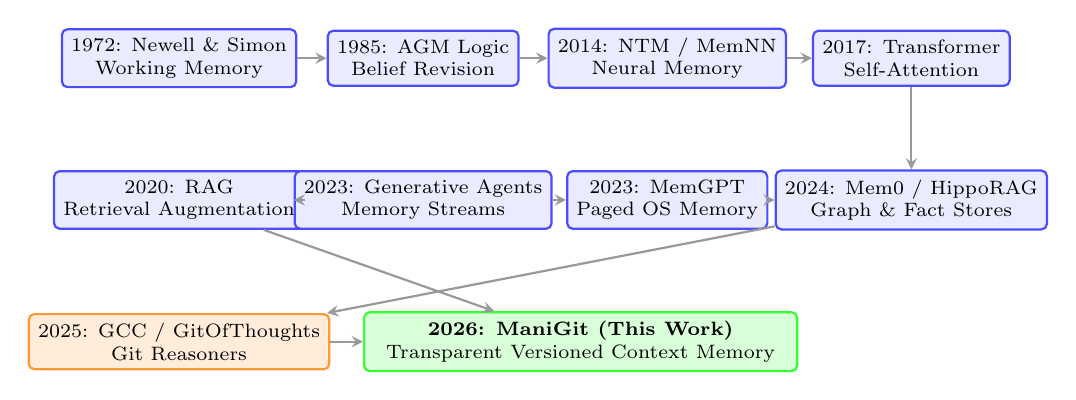
\begin{tikzpicture}[node distance=1.3cm, auto,
    every node/.style={font=\scriptsize},
    stage/.style={rectangle, draw=blue!70, fill=blue!8, thick, minimum width=2.4cm, minimum height=0.7cm, align=center, rounded corners=2pt},
    arrow/.style={->, >=stealth, thick, color=gray!80}]

\node[stage] (s1) {1972: Newell \& Simon\\Working Memory};
\node[stage, right of=s1, xshift=1.8cm] (s2) {1985: AGM Logic\\Belief Revision};
\node[stage, right of=s2, xshift=1.8cm] (s3) {2014: NTM / MemNN\\Neural Memory};
\node[stage, right of=s3, xshift=1.8cm] (s4) {2017: Transformer\\Self-Attention};

\node[stage, below of=s1, yshift=-0.5cm] (s5) {2020: RAG\\Retrieval Augmentation};
\node[stage, right of=s5, xshift=1.8cm] (s6) {2023: Generative Agents\\Memory Streams};
\node[stage, right of=s6, xshift=1.8cm] (s7) {2023: MemGPT\\Paged OS Memory};
\node[stage, right of=s7, xshift=1.8cm] (s8) {2024: Mem0 / HippoRAG\\Graph \& Fact Stores};

\node[stage, below of=s5, yshift=-0.5cm, fill=orange!15, draw=orange!80] (s9) {2025: GCC / GitOfThoughts\\Git Reasoners};
\node[stage, right of=s9, xshift=3.8cm, fill=green!15, draw=green!80, minimum width=5.5cm] (s10) {\textbf{2026: ManiGit (This Work)}\\Transparent Versioned Context Memory};

\draw[arrow] (s1) -- (s2);
\draw[arrow] (s2) -- (s3);
\draw[arrow] (s3) -- (s4);
\draw[arrow] (s4) -- (s8);
\draw[arrow] (s5) -- (s6);
\draw[arrow] (s6) -- (s7);
\draw[arrow] (s7) -- (s8);
\draw[arrow] (s8) -- (s9);
\draw[arrow] (s9) -- (s10);
\draw[arrow] (s5) -- (s10);

\end{tikzpicture}%
}

\caption{Historical evolution of agent memory architectures from classical AI production systems (1972) and formal belief revision (1985) to differentiable neural memory, retrieval-augmented generation, operating-system-inspired paging, and transparent versioned context memory.}
\label{fig:history_timeline}
\end{figure*}

\subsection{Foundations: Production Rules and Belief Revision}
The conceptual separation between bounded working memory and persistent long-term knowledge traces back to Newell and Simon's seminal work on human problem solving~\cite{newell1972human}. Production systems formalized memory as an active working memory buffer holding immediate goal chunks, interacting with a persistent repository of declarative rules. However, classical production systems relied on manual symbolic engineering and lacked natural language adaptability.

Concurrently, the philosophical and mathematical foundations of memory updating were established by Alchourr{\'o}n, G{\"a}rdenfors, and Makinson~\cite{agm1985logic} in the AGM belief revision framework. AGM formalized the logical postulates of \textit{Success} (incorporating new facts), \textit{Consistency} (avoiding contradictory states), and \textit{Minimal Change} (minimizing information loss during contraction). While theoretically rigorous, classical belief revision was computationally intractable for open-domain natural language and modeled belief contraction destructively, erasing retracted propositions from active consideration.

\subsection{Differentiable Neural Memory}
In the deep learning era, researchers attempted to augment recurrent neural networks with external continuous memory arrays. Graves et al.~\cite{graves2014neural} introduced \textit{Neural Turing Machines} (NTM), enabling networks to read and write to continuous memory matrices via differentiable addressing. Weston et al.~\cite{weston2014memory} proposed \textit{Memory Networks}, using continuous memory slot arrays to execute multi-hop reasoning over synthetic question-answering tasks. Graves et al.~\cite{graves2016hybrid} advanced this with the \textit{Differentiable Neural Computer} (DNC), incorporating a temporal link matrix to track the chronological sequence of memory allocations. While foundational, differentiable neural computers proved notoriously difficult to optimize and could not scale to open-domain natural language dialogues.

\subsection{RAG and Conversational Buffers}
The rise of large pre-trained language models shifted the memory paradigm toward non-parametric retrieval. REALM~\cite{guu2020realm} and RAG~\cite{lewis2020retrieval} established dense passage retrieval as the dominant mechanism for externalizing knowledge without fine-tuning model parameters. In conversational settings, early assistant implementations introduced sliding conversation buffers and running summaries. However, as demonstrated in our experiments, sliding windows drop foundational instructions when dialogue exceeds buffer length, while running summaries irreversibly discard exact technical constraints through lossy paraphrase.

\subsection{Modern Persistent Agent Memory Systems}
Over the past three years, persistent agent memory has become an active frontier:
\begin{itemize}
    \item \textbf{Cognitive and Reflection Streams:} Park et al.~\cite{park2023generative} demonstrated that simulated agents could maintain multi-day social relationships using an append-only memory stream scored by recency, importance, and relevance, paired with periodic synthetic reflection. Zhong et al.~\cite{zhong2023memorybank} introduced \textit{MemoryBank}, applying an exponential Ebbinghaus forgetting curve to prioritize recently reinforced memories.
    \item \textbf{Operating-System Architectures:} Packer et al.~\cite{packer2023memgpt} introduced \textit{MemGPT}, treating the context window as RAM and external databases as disk, managed through explicit LLM tool calls. Kang et al.~\cite{kang2025memoryos} formalized operating-system-inspired memory hierarchies for LLM agents, structuring memory across short-term, mid-term, and persistent tiers.
    \item \textbf{Graph and Networked Memory:} Guti{\'e}rrez et al.~\cite{gutierrez2024hipporag} developed \textit{HippoRAG}, mimicking mammalian hippocampal indexing via Personalized PageRank over knowledge graphs. Edge et al.~\cite{edge2024graphrag} introduced \textit{Graph RAG}, using graph community detection for hierarchical corpus summarization. Xu et al.~\cite{xu2024amem} proposed \textit{A-MEM}, structuring memories into Zettelkasten-style interconnected note networks.
    \item \textbf{Commercial Fact Stores:} Deshmukh et al.~\cite{deshmukh2024mem0} developed \textit{Mem0}, providing a multi-scope memory orchestration layer (user, session, agent) with hybrid vector-graph backends.
\end{itemize}

\subsection{Emergence of Git Metaphors in Agent State}
Most recently, researchers have explored applying Git-like version control metaphors to LLM agents:
\begin{itemize}
    \item \textbf{Git Context Controller (GCC):} Wu et al.~\cite{wu2025gcc} proposed GCC, equipping software engineering agents on SWE-bench with explicit commands (\texttt{COMMIT}, \texttt{BRANCH}, \texttt{MERGE}, \texttt{CONTEXT}) to manage Markdown notes in a local workspace directory.
    \item \textbf{GitOfThoughts:} Shekar et al.~\cite{shekar2025gitofthoughts} introduced GitOfThoughts, mapping tree-of-thoughts reasoning paths into native Git commits for mathematical problem solving.
\end{itemize}

As analyzed in Section~\ref{sec:research_gap}, while GCC and GitOfThoughts validate the conceptual appeal of Git for agent workflows, both systems require the agent to manually execute version-control tool calls, lack automated memory intake classification, do not maintain functional memory tiers, and lack budget-constrained knapsack context compilation.

\section{Research Gap and Novelty Positioning}
\label{sec:research_gap}

A systematic analysis of our literature corpus (encompassing 34 foundational and contemporary studies across cognitive architectures, external memory networks, agent memory stores, and context management frameworks) reveals five critical, unaddressed gaps that limit the reliability and auditability of long-running autonomous agents. Among the 34 papers reviewed in our literature corpus, only 5 (14.7\%) explore any versioning concepts, and none integrate automated DAG commit tracking with budget-constrained knapsack context compilation.

\subsection{Gap 1: Destructive Mutation vs. Immutable Versioning}
In mainstream persistent agent memory architectures (e.g., MemGPT~\cite{packer2023memgpt}, Mem0~\cite{deshmukh2024mem0}), memory updates are executed as destructive in-place text replacements or SQL \texttt{UPDATE}/\texttt{DELETE} operations. Once modified, prior states are obliterated. If an agent misbehaves or suffers a prompt injection attack, developers cannot reconstruct the agent's exact epistemic state at that moment.

\textit{Counterexample Analysis:} Git Context Controller (GCC)~\cite{wu2025gcc} and GitOfThoughts~\cite{shekar2025gitofthoughts} use Git commits, but require the LLM itself to manually invoke tool commands to write and commit notes. This imposes significant token overhead and relies on the model remembering to manage its own version control. In contrast, ManiGit provides an \textbf{automated, transparent infrastructure layer}: incoming messages are automatically parsed, classified, and committed to an immutable commit DAG in SQLite without requiring agent tool calls or prompt tokens.

\subsection{Gap 2: Contradiction Handling and Ghost Context}
In vector-based memory systems, text chunks are indexed as timeless semantic points. When user constraints change across sessions (e.g., migrating from PostgreSQL to MongoDB), vector similarity search retrieves both the obsolete initial choice and the new requirement. This introduces \textit{ghost context} into the prompt, forcing the language model to arbitrate conflicting premises. Recent evaluations on STALE~\cite{stale2025benchmark} and LongMemEval~\cite{wu2024longmemeval} confirm that frontier models fail on implicit contradictory premises in over 40\% of trials.

\textit{Partial Solutions:} Generative Agents~\cite{park2023generative} applies recency weighting, which merely dampens older memories without removing them. MemoryBank~\cite{zhong2023memorybank} applies exponential decay based on time rather than logical contradiction. In contrast, ManiGit implements \textbf{explicit contradiction detection and supersession}. When a new fact is ingested, active memories are evaluated for semantic conflict. Superseded facts are automatically transitioned to the \texttt{ARCHIVED} tier, removing them from active prompt compilation while preserving their provenance in the commit graph.

\subsection{Gap 3: Point-in-Time Historical Reconstruction}
When auditing long-running agents or answering retrospective questions (e.g., ``What was our deployment target prior to commit $C_k$?''), existing persistent systems evaluated in our literature review generally do not provide the combination of versioned memory state and point-in-time reconstruction, as past states have either been overwritten or blurred into an uncurated flat log.

\textit{Counterexample Analysis:} While Git provides checkout semantics for source code, prior agent architectures do not provide point-in-time state reconstruction for conversational context memory under budget constraints. ManiGit provides \textbf{first-class historical checkout}: given any historical commit hash $C_k$, ManiGit reconstructs the exact active memory set as it existed at $C_k$ and compiles a budget-compliant context window for that exact historical moment, achieving 100\% recovery accuracy across the evaluated benchmark checkout scenarios.

\subsection{Gap 4: Token-Budget Context Compilation (Memory $\ne$ Context)}
Existing systems frequently conflate persistent memory storage with prompt context assembly. Naive in-context approaches stuff as many retrieved chunks as possible until prompt limits are reached. However, empirical studies confirm that long, bloated contexts degrade model attention~\cite{liu2024lost,dong2023bamboo}.

\textit{Counterexample Analysis:} Classic information retrieval has formulated sentence extraction as a knapsack problem for multi-document summarization, but has not integrated it with dynamic, versioned memory tiers. ManiGit formalizes context construction as a \textbf{bounded knapsack optimization problem} subject to a hard token budget $B$:
\begin{equation}
\max_{C_t \subseteq \mathcal{M}_t} \sum_{m_i \in C_t} U(m_i, q_t) \quad \text{subject to} \quad \sum_{m_i \in C_t} L(m_i) \le B
\end{equation}
ManiGit addresses this via a deterministic greedy score-density compiler that balances query relevance, composite priority, and memory tier weighting, maintaining zero budget violations ($\sum_{m_i \in C_t} L(m_i) \le B$) across all evaluated trials.

\subsection{Gap 5: Provenance and Auditable Why Reports}
When an agent acts on a stored memory, standard vector stores offer no visibility into why the fact was retained, which user message generated it, or what confidence score was assigned.

\textit{ManiGit Positioning:} Every memory fact in ManiGit maintains bidirectional pointers to the originating raw message ID and turn index, accompanied by a structured \textbf{Why Report} documenting the classification rule, LLM judge confidence score, and supersession target.

\section{ManiGit Architecture}
\label{sec:manigit_architecture}

ManiGit is designed as a modular, transparent infrastructure layer situated between the raw conversational dialogue stream and the LLM inference runtime. Fig.~\ref{fig:architecture} illustrates the overall system architecture, and Fig.~\ref{fig:memory_lifecycle} details the memory lifecycle state machine.

\begin{figure*}[t]
\centering
\resizebox{0.95\textwidth}{!}{%
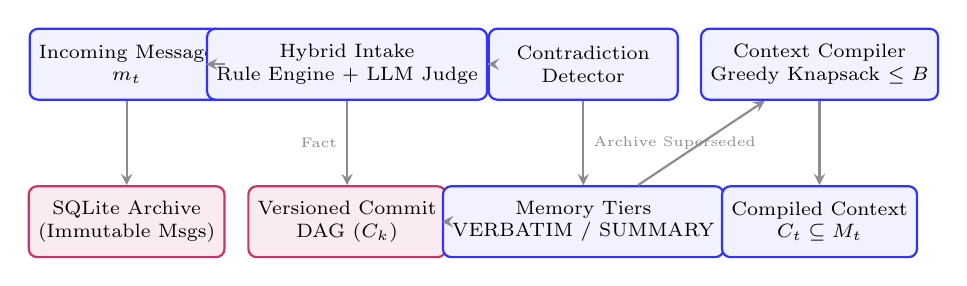
\begin{tikzpicture}[
    box/.style={rectangle, draw=blue!80, fill=blue!5, thick, rounded corners=3pt, minimum width=2.4cm, minimum height=0.9cm, align=center, font=\scriptsize},
    databox/.style={rectangle, draw=purple!80, fill=purple!8, thick, rounded corners=3pt, minimum width=2.4cm, minimum height=0.9cm, align=center, font=\scriptsize},
    flow/.style={->, >=stealth, thick, color=gray!90}]

\node[box] (msg) {Incoming Message\\$m_t$};
\node[box, right of=msg, xshift=1.8cm] (class) {Hybrid Intake\\Rule Engine + LLM Judge};
\node[databox, below of=msg, yshift=-1.0cm] (rawdb) {SQLite Archive\\(Immutable Msgs)};
\node[databox, right of=rawdb, xshift=1.8cm] (dag) {Versioned Commit\\DAG ($C_k$)};
\node[box, right of=class, xshift=2.0cm] (contra) {Contradiction\\Detector};
\node[box, right of=dag, xshift=2.0cm] (tiers) {Memory Tiers\\VERBATIM / SUMMARY};
\node[box, right of=contra, xshift=2.0cm] (compiler) {Context Compiler\\Greedy Knapsack $\le B$};
\node[box, below of=compiler, yshift=-1.0cm] (prompt) {Compiled Context\\$C_t \subseteq M_t$};

\draw[flow] (msg) -- (class);
\draw[flow] (msg) -- (rawdb);
\draw[flow] (class) -- node[left, font=\tiny]{Fact} (dag);
\draw[flow] (class) -- (contra);
\draw[flow] (contra) -- node[right, font=\tiny]{Archive Superseded} (tiers);
\draw[flow] (dag) -- (tiers);
\draw[flow] (tiers) -- (compiler);
\draw[flow] (compiler) -- (prompt);

\end{tikzpicture}%
}

\caption{ManiGit system architecture: Raw messages are stored immutably in SQLite. The hybrid intake pipeline classifies candidate facts into functional tiers and commits them to the versioned DAG. The contradiction detector identifies superseding facts, archiving older versions and recording Why Reports. The context compiler executes a greedy knapsack selection over active memories to assemble a budget-constrained context window $C_t \le B$ for the model adapter.}
\label{fig:architecture}
\end{figure*}

\begin{figure}[t]
\centering
\resizebox{0.92\columnwidth}{!}{%
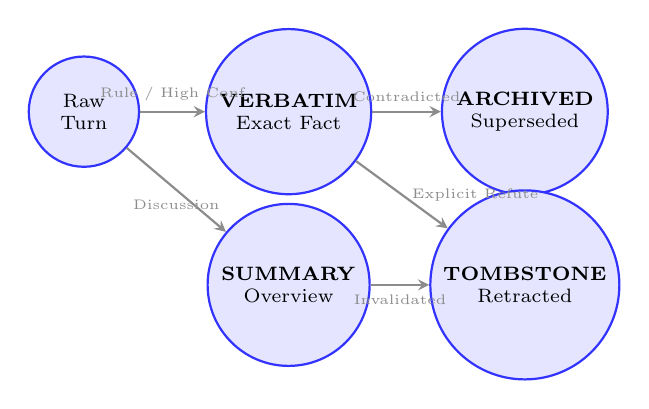
\begin{tikzpicture}[
    state/.style={circle, draw=blue!80, fill=blue!10, thick, minimum size=1.4cm, align=center, font=\scriptsize},
    trans/.style={->, >=stealth, thick, color=gray!90}]

\node[state] (raw) {Raw\\Turn};
\node[state, right of=raw, xshift=1.6cm] (verb) {\textbf{VERBATIM}\\Exact Fact};
\node[state, below of=verb, yshift=-1.2cm] (summ) {\textbf{SUMMARY}\\Overview};
\node[state, right of=verb, xshift=2.0cm] (arch) {\textbf{ARCHIVED}\\Superseded};
\node[state, right of=summ, xshift=2.0cm] (tomb) {\textbf{TOMBSTONE}\\Retracted};

\draw[trans] (raw) -- node[above, font=\tiny]{Rule / High Conf} (verb);
\draw[trans] (raw) -- node[below, font=\tiny]{Discussion} (summ);
\draw[trans] (verb) -- node[above, font=\tiny]{Contradicted} (arch);
\draw[trans] (summ) -- node[below, font=\tiny]{Invalidated} (tomb);
\draw[trans] (verb) -- node[right, font=\tiny]{Explicit Refute} (tomb);

\end{tikzpicture}%
}

\caption{ManiGit four-tier memory lifecycle state machine. Raw dialogue turns transition into \texttt{VERBATIM} (exact constraints/decisions) or \texttt{SUMMARY} (high-level overviews). When contradicted, facts transition to \texttt{ARCHIVED}; explicit refutations transition facts to \texttt{TOMBSTONE}.}
\label{fig:memory_lifecycle}
\end{figure}

\subsection{Immutable Message Archive}
All incoming raw messages $m_t$ (from both user and assistant turns) are appended directly to an immutable SQLite repository. Each record stores:
$$\text{Record}(m_t) = \langle \text{id}, \text{session\_id}, \text{role}, \text{content}, \text{timestamp}, \text{content\_hash} \rangle$$
where $\text{content\_hash}$ is computed via SHA-256 over normalized message content. Messages cannot be mutated or deleted under any circumstance, establishing an immutable, content-addressed ground truth.

\subsection{Hybrid Rule-First Memory Classification}
Raw conversational turns contain a mixture of casual dialogue, transient pleasantries, and critical technical instructions. Storing every turn as a memory fact causes memory bloat; conversely, running an LLM on every turn introduces severe latency.

ManiGit implements a two-stage hybrid intake pipeline:
\begin{enumerate}
    \item \textbf{Rule Engine (Stage 1):} Evaluates incoming turns against deterministic regex pattern rules targeting high-priority signals (explicit constraints, database selections, credentials, API endpoints). If a rule matches, the fact is immediately classified into the \texttt{VERBATIM} tier with maximum confidence ($c = 1.0$) and zero API latency.
    \item \textbf{LLM Judge (Stage 2):} Turns not matching deterministic rules fall through to an LLM judge calibrated with explicit confidence thresholds:
    $$\text{Tier}(f) = \begin{cases}
    \texttt{VERBATIM}, & \text{if } c \ge 0.85 \text{ and is\_constraint}(f) \\
    \texttt{SUMMARY},  & \text{if } c \ge 0.70 \text{ and is\_discussion}(f) \\
    \texttt{ARCHIVED}, & \text{if } c < 0.70 \text{ (speculative / uncertain)}
    \end{cases}$$
\end{enumerate}

\subsection{Versioned Commit DAG}
Instead of updating memory records in place, ManiGit models memory states as commits in a Directed Acyclic Graph (DAG). A commit $C_k$ encapsulates:
$$C_k = \langle \text{commit\_hash}, \text{parent\_hash}, \text{branch}, \text{message}, \text{timestamp}, \mathcal{M}_k \rangle$$
where $\mathcal{M}_k = \{m_1, m_2, \dots, m_n\}$ denotes the set of active memory objects valid at that commit. Commits are linked via SHA-256 parent hashes, exactly mirroring Git repository semantics. Branch isolation enables agents to explore alternative reasoning branches without contaminating the production memory branch.

\subsection{Bidirectional Provenance & Why Reports}
Every memory object $m_i \in \mathcal{M}_k$ maintains explicit bidirectional provenance:
\begin{itemize}
    \item \textbf{Source Linkage:} Pointers to the originating message ID ($\text{source\_msg\_id}$) and turn index.
    \item \textbf{Why Report:} A structured audit document recording:
    $$\text{WhyReport}(m_i) = \langle \text{rule\_id}, \text{judge\_confidence}, \text{decision\_rationale}, \text{superseded\_target\_id} \rangle$$
\end{itemize}
This ensures that any memory accessed during context compilation can be directly traced back to its originating conversation turn and classification rationale via explicit relational provenance links.

\subsection{Automated Contradiction Detection & Supersession}
When a new memory fact $m_{\text{new}}$ is classified, ManiGit executes semantic conflict detection against all active memories in the current branch. If $m_{\text{new}}$ supersedes or contradicts an active fact $m_{\text{old}}$:
\begin{enumerate}
    \item $m_{\text{old}}$ is transitioned from its current tier to \texttt{ARCHIVED}.
    \item The supersession relationship is recorded in $m_{\text{new}}$'s Why Report ($\text{supersedes} = m_{\text{old}}.\text{id}$).
    \item A new commit $C_{k+1}$ is generated where $\mathcal{M}_{k+1} = (\mathcal{M}_k \setminus \{m_{\text{old}}\}) \cup \{m_{\text{new}}\}$.
\end{enumerate}
Because $m_{\text{old}}$ is archived rather than deleted, it is completely removed from subsequent prompt context compilation, preventing ghost context while remaining fully recoverable in historical commit states.

\subsection{Context Compilation under Token Budgets}
When the agent receives a user query $q_t$, the Context Compiler dynamically selects a subset of active memories $C_t \subseteq \mathcal{M}_k$ that maximizes relevance while strictly adhering to a pre-allocated token budget $B$. The formal mathematical optimization and greedy knapsack compilation are detailed in Section~\ref{sec:mathematical_formulation}.

\subsection{Point-in-Time Historical Reconstruction}
ManiGit supports deterministic time travel. By invoking:
$$\text{checkout}(C_{\text{target}})$$
the Context Compiler reconstructs the exact active memory set $\mathcal{M}_{\text{target}}$ as it existed at commit $C_{\text{target}}$ and compiles a budget-compliant context window for that past moment. This enables agents to answer historical retrospective questions deterministically without polluting current branch state, achieving 100\% point-in-time reconstruction across evaluated benchmark scenarios.

\section{Mathematical Formulation}
\label{sec:mathematical_formulation}

ManiGit establishes a formal mathematical separation between \textit{memory storage} and \textit{context compilation}. While memory storage $\mathcal{M}_t$ accumulates monotonically across an agent's lifecycle, the operative context window $C_t$ assembled for query $q_t$ must respect a strict token budget $B$. Fig.~\ref{fig:context_compilation} illustrates the budget-constrained context selection problem.

\begin{figure}[t]
\centering
\resizebox{0.98\columnwidth}{!}{%
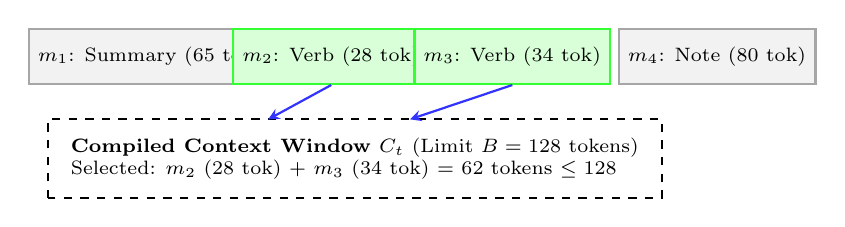
\begin{tikzpicture}[
    item/.style={rectangle, draw=gray!70, fill=gray!10, thick, minimum height=0.7cm, align=center, font=\scriptsize},
    active/.style={rectangle, draw=green!80, fill=green!15, thick, minimum height=0.7cm, align=center, font=\scriptsize},
    flow/.style={->, >=stealth, thick, color=blue!80}]

\node[item, minimum width=2.2cm] (m1) {$m_1$: Summary (65 tok)};
\node[active, minimum width=1.5cm, right of=m1, xshift=1.3cm] (m2) {$m_2$: Verb (28 tok)};
\node[active, minimum width=1.8cm, right of=m2, xshift=1.3cm] (m3) {$m_3$: Verb (34 tok)};
\node[item, minimum width=2.5cm, right of=m3, xshift=1.6cm] (m4) {$m_4$: Note (80 tok)};

\draw[draw=black, dashed, thick] (-1.3, -1.8) rectangle (6.5, -0.8);
\node[font=\scriptsize, align=left] at (2.6, -1.3) {\textbf{Compiled Context Window $C_t$} (Limit $B=128$ tokens)\\Selected: $m_2$ (28 tok) + $m_3$ (34 tok) = 62 tokens $\le 128$};

\draw[flow] (m2.south) -- (1.5, -0.8);
\draw[flow] (m3.south) -- (3.3, -0.8);

\end{tikzpicture}%
}

\caption{Mathematical knapsack formulation of context compilation. Memory objects are ranked by utility density $D(m_i,q_t)=U(m_i,q_t)/L(m_i)$ and selected under the hard token budget $B$.}
\label{fig:context_compilation}
\end{figure}

\subsection{Formal Optimization Problem}
Let $\mathcal{M}_t = \{m_1, m_2, \dots, m_N\}$ be the set of active memory objects in the current branch at turn $t$. Each memory object $m_i$ possesses:
\begin{itemize}
    \item A token length $L(m_i) \in \mathbb{N}^+$, measured via deterministic tokenization.
    \item A functional tier $\tau(m_i) \in \{\texttt{VERBATIM}, \texttt{SUMMARY}, \texttt{ARCHIVED}, \texttt{TOMBSTONE}\}$.
    \item An intrinsic priority weight $p(m_i) \in [0, 1]$.
    \item An age or creation timestamp $t(m_i)$.
\end{itemize}

Given an incoming user query $q_t$ and a hard pre-allocated token budget $B \in \mathbb{N}^+$, the context compilation objective is to select an optimal subset $C_t^* \subseteq \mathcal{M}_t$ such that:
\begin{equation}
C_t^* = \arg\max_{C_t \subseteq \mathcal{M}_t} \sum_{m_i \in C_t} U(m_i, q_t)
\label{eq:knapsack_obj}
\end{equation}
subject to the hard budget constraint:
\begin{equation}
\sum_{m_i \in C_t} L(m_i) \le B
\label{eq:knapsack_constraint}
\end{equation}
where only active memories are eligible for selection ($\tau(m_i) \in \{\texttt{VERBATIM}, \texttt{SUMMARY}\}$).

\subsection{Composite Utility Function}
The utility $U(m_i, q_t)$ evaluates the suitability of memory $m_i$ for query $q_t$ as a convex combination of relevance, tier boost, and priority:
\begin{equation}
U(m_i, q_t) = w_{\text{rel}} \cdot R(m_i, q_t) + w_{\text{tier}} \cdot T(m_i) + w_{\text{prio}} \cdot p(m_i)
\label{eq:utility}
\end{equation}
where:
\begin{itemize}
    \item $R(m_i, q_t) \in [0, 1]$ is the normalized lexical relevance score between query $q_t$ and memory content $m_i$, computed via Okapi BM25 and term overlap:
    $$R(m_i, q_t) = \frac{\text{BM25}(m_i, q_t)}{\max_{m_j \in \mathcal{M}_t} \text{BM25}(m_j, q_t) + \epsilon}$$
    \item $T(m_i) \in [0, 1]$ is the tier-specific preference multiplier:
    $$T(m_i) = \begin{cases}
    1.0, & \text{if } \tau(m_i) = \texttt{VERBATIM} \\
    0.7, & \text{if } \tau(m_i) = \texttt{SUMMARY} \\
    0.0, & \text{otherwise}
    \end{cases}$$
    \item $p(m_i) \in [0, 1]$ is the intrinsic priority assigned during intake (e.g., $1.0$ for security credentials, $0.8$ for architecture choices, $0.5$ for conversational summaries).
    \item $w_{\text{rel}} = 0.5$, $w_{\text{tier}} = 0.3$, and $w_{\text{prio}} = 0.2$ are normalized mixture weights summing to $1.0$.
\end{itemize}

\subsection{Greedy Knapsack Approximation Algorithm}
The optimization problem defined in Equations~\eqref{eq:knapsack_obj} and~\eqref{eq:knapsack_constraint} is isomorphic to the classic 0-1 Knapsack Problem, which is known to be NP-hard. ManiGit does not solve the exact combinatorial optimization problem at inference time; instead, this formulation motivates our practical system design, which uses local lexical retrieval, tier/confidence/priority scoring signals, and a deterministic greedy score-density selection algorithm:

\begin{enumerate}
    \item \textbf{Density Calculation:} For every active memory $m_i \in \mathcal{M}_t$, compute its utility density per token:
    \begin{equation}
    D(m_i, q_t) = \frac{U(m_i, q_t)}{L(m_i)}
    \end{equation}
    \item \textbf{Sorting:} Sort candidate memories in descending order of density:
    \begin{equation}
    D(m_{(1)}, q_t) \ge D(m_{(2)}, q_t) \ge \dots \ge D(m_{(N)}, q_t)
    \end{equation}
    \item \textbf{Greedy Packing:} Initialize $C_t \leftarrow \emptyset$ and accumulated tokens $K \leftarrow 0$. For each sorted candidate $m_{(i)}$:
    \begin{equation}
    \begin{aligned}
    &\text{if } K + L(m_{(i)}) \le B\text{ then} \\
    &\quad C_t \leftarrow C_t \cup \{m_{(i)}\}, \quad K \leftarrow K + L(m_{(i)})
    \end{aligned}
    \end{equation}
    \item \textbf{Early Termination:} Stop when no remaining candidate fits within the residual budget $B - K$.
\end{enumerate}

\subsection{Theoretical Guarantee: Memory $\ne$ Context}
This formulation guarantees two critical invariants:
\begin{enumerate}
    \item \textbf{Budget Invariance:} $\sum_{m_i \in C_t} L(m_i) \le B$ holds strictly for all $t$ and all queries, ensuring that agent prompts never exceed allocated token budgets or trigger LLM context overflow errors.
    \item \textbf{Decoupled Scalability:} The total size of persistent memory $|\mathcal{M}_t|$ can grow indefinitely without expanding the active context size $|C_t|$, successfully decoupling agent operational longevity from model inference cost.
\end{enumerate}

\section{Experimental Methodology}
\label{sec:methodology}

Our experimental evaluation is designed to answer the central research question: \textit{Which components of ManiGit contribute to memory quality, historical correctness, contradiction handling, provenance, and budget-aware context selection?}

\subsection{Research Hypotheses}
We formalize five explicit research hypotheses:
\begin{itemize}
    \item \textbf{H1 (Budget Robustness):} ManiGit Full maintains comparable or higher factual recall and answer correctness relative to non-versioned baselines while consuming significantly fewer context tokens under constrained budgets.
    \item \textbf{H2 (Historical Reconstruction):} ManiGit's versioned commit DAG enables reliable point-in-time state recovery of previously valid facts after supersession, where baselines fail.
    \item \textbf{H3 (Contradiction Adjudication):} Automated contradiction supersession materially improves answer correctness on scenarios involving changing requirements.
    \item \textbf{H4 (Confidence Awareness):} Confidence-calibrated classification improves agent robustness on ambiguous or speculative memory statements.
    \item \textbf{H5 (Tier Selection Boost):} Tier-aware ranking improves factual recall under tight token budgets ($B=128$) when concise constraints compete with verbose summaries.
\end{itemize}

\subsection{Experimental Design and Matrix Cardinality}
\begin{equation}
\begin{aligned}
\text{Total Trials} &= 22\text{ queries} \times 8\text{ methods} \times 5\text{ budgets} \\
&= 880\text{ raw experimental trials}
\end{aligned}
\end{equation}
Budgets evaluate the operational spectrum from constrained to unconstrained contexts:
$$B \in \{128, 256, 512, 1024, 2048\}\text{ tokens}$$
To ensure statistical validity, the unit of analysis is defined as the \textbf{query-budget pair} ($N = 22 \times 5 = 110$ evaluation pairs per method). We explicitly do not treat these 110 pairs as 110 independent conversations.

\subsection{Comparative Baselines}
We compare ManiGit Full against four established context management strategies:
\begin{enumerate}
    \item \textbf{Full History:} Ingests all preceding conversational turns into the prompt until budget $B$ is reached, truncating earlier turns if necessary. Represents the standard in-context memory paradigm.
    \item \textbf{Sliding Window ($N=10$):} Retains strictly the most recent 10 conversational turns, discarding older history regardless of semantic significance.
    \item \textbf{Running Summary:} Progressively compresses historical dialogue into an ongoing natural language summary preamble using recursive text aggregation.
    \item \textbf{RAG-Style Retrieval:} Indexes raw message turns in an external lexical/vector store and retrieves top-$k$ segments matching query $q_t$ within budget $B$.
\end{enumerate}

\subsection{Controlled Ablation Variants}
To isolate the causal contribution of individual ManiGit mechanisms, we implement three controlled ablations where exactly one mechanism is neutralized while holding all other components identical:
\begin{enumerate}
    \item \textbf{ManiGit (no\_contradiction):} Contradiction detection is disabled via an evaluation adapter. Superseded facts remain active in memory alongside new facts, directly measuring the vulnerability to ghost context.
    \item \textbf{ManiGit (no\_confidence):} Confidence calibration is neutralized; candidate assertions are classified without confidence awareness, demonstrating the impact of premature archiving.
    \item \textbf{ManiGit (no\_tier):} Memory tier multipliers ($T(m_i)$) are set to $1.0$ for all active tiers, removing preference for concise verbatim facts over verbose summaries during knapsack compilation.
\end{enumerate}

\subsection{Scenario Matrix}
The benchmark comprises 11 multi-turn scenarios spanning distinct operational challenges:
\begin{enumerate}
    \item \textit{Stable Factual Memory:} Foundational user facts that remain constant across all turns.
    \item \textit{Superseding Facts (PostgreSQL $\to$ MongoDB):} Technical migration where an early database selection is explicitly reversed in a later session.
    \item \textit{Exact Technical Constraints:} Strict port numbers, timeout limits, and memory thresholds requiring exact verbatim recall.
    \item \textit{Architectural Decisions:} High-level system design trade-offs.
    \item \textit{Conversational Distractors:} Off-topic casual banter designed to trigger false-positive memory ingestion.
    \item \textit{Duplicate Assertions:} Re-stated facts testing deduplication resilience.
    \item \textit{Extended Dialogue Sequences:} Long conversations testing context accumulation.
    \item \textit{Point-in-Time Reconstruction:} Retrospective queries asking what configuration was valid at an earlier commit hash $C_k$.
    \item \textit{Branch Isolation:} Parallel exploratory branches with conflicting parameters.
    \item \textit{Ambiguous Confidence:} Speculative statements (``We might scale to 10 nodes, but it is tentative'') probing confidence-calibrated intake.
    \item \textit{Tier Selection Competition:} Tight budget ($B=128$) where a concise verbatim constraint competes for space against a verbose summary overview.
\end{enumerate}
Each scenario features 2 mutually exclusive queries (1 testing current active state, 1 testing historical or past state), yielding 22 queries total.

\subsection{Evaluation Metrics}
\begin{itemize}
    \item \textbf{Fact Recall (\%):} Binary metric indicating whether all ground-truth target facts required for query $q_t$ are present in the compiled context $C_t$.
    \item \textbf{Answer Correctness (\%):} Binary metric indicating whether the model adapter generates a semantically correct answer matching ground truth.
    \item \textbf{Historical Recovery (\%):} Accuracy on retrospective queries evaluated against past commit states.
    \item \textbf{Context Tokens:} Actual number of prompt tokens consumed by compiled context $C_t$.
    \item \textbf{Budget Compliance (\%):} Percentage of trials satisfying the strict inequality $\sum L(m_i) \le B$.
    \item \textbf{Latency (ms):} Wall-clock time required for memory classification, commit insertion, and context compilation.
\end{itemize}

\subsection{Statistical Methodology}
For binary metrics (Fact Recall, Answer Correctness, Historical Recovery), we compute exact \textbf{95\% Wilson score confidence intervals} without continuity correction:
\begin{equation}
\tilde{p} = \frac{k + \frac{z^2}{2}}{n + z^2}, \quad \text{CI} = \tilde{p} \pm \frac{z}{n + z^2} \sqrt{\frac{k(n-k)}{n} + \frac{z^2}{4}}
\end{equation}
with $z = 1.96$ and $n = 110$. Continuous token metrics are reported as sample mean $\pm$ sample standard deviation ($\sigma$). For comparative ablation analysis, we report paired differences across identical $(q_t, B)$ evaluation pairs ($N = 110$ pairs per ablation).

\subsection{Fairness and Isolation Controls}
All 8 methods receive the exact same source conversations, identical queries, identical token budgets, and deterministic mock model adapters with fixed random seed 42. No method receives privileged hints or hardcoded answers. All trials run against isolated in-memory or temporary SQLite repositories, guaranteeing zero cross-trial data leakage.

\section{Experimental Results}
\label{sec:results}

We report empirical findings across 880 experimental trials ($N=110$ trials per method across 5 budgets). Table~\ref{tab:overall_comparison} summarizes overall comparative performance, and Table~\ref{tab:budget_breakdown} details performance broken down by individual token budgets.

\begin{table*}[t]
\centering
\caption{Overall comparative performance across all 880 trials ($N=110$ trials per method across 5 budgets: 128, 256, 512, 1024, 2048). Fact Recall includes 95\% Wilson score confidence intervals. Context Tokens reported as sample mean $\pm$ standard deviation.}
\label{tab:overall_comparison}
\setlength{\tabcolsep}{4.2pt}
\resizebox{\textwidth}{!}{%
\begin{tabular}{lcccccccc}
\toprule
\textbf{Method} & \textbf{Fact Recall} & \textbf{95\% CI} & \textbf{Ans. Corr.} & \textbf{Hist. Rec.} & \textbf{Context Tok.} & \textbf{Total Tok.} & \textbf{Retr. Prec.} & \textbf{Latency (ms)} \\
\midrule
Full History               & 83.6\% & [75.6\%, 89.4\%] & 79.1\% & 100.0\% & $298.4 \pm 374.1$ & 323.3 & 0.230 & 0.04 \\
ManiGit (Full)             & 86.4\% & [78.7\%, 91.6\%] & 86.4\% & 100.0\% & $170.2 \pm 221.9$ & 194.9 & 0.270 & 0.98 \\
ManiGit (no\_confidence)   & 81.8\% & [73.6\%, 87.9\%] & 81.8\% & 100.0\% & $169.2 \pm 222.5$ & 194.2 & 0.250 & 0.92 \\
ManiGit (no\_contradiction)& 86.4\% & [78.7\%, 91.6\%] & 81.8\% & 100.0\% & $170.7 \pm 221.7$ & 196.1 & 0.260 & 1.11 \\
ManiGit (no\_tier)         & 85.5\% & [77.7\%, 90.8\%] & 85.5\% & 100.0\% & $171.0 \pm 221.6$ & 195.8 & 0.260 & 0.96 \\
RAG-Style (Raw Messages)   & 95.5\% & [89.8\%, 98.0\%] & 90.9\% & 100.0\% & $188.7 \pm 191.9$ & 213.3 & 0.390 & 0.52 \\
Running Summary            & 95.5\% & [89.8\%, 98.0\%] & 86.4\% & 100.0\% & $33.4 \pm 11.5$   & 58.5  & 0.470 & 0.01 \\
Sliding Window ($N=10$)    & 76.4\% & [67.6\%, 83.3\%] & 71.8\% & 100.0\% & $136.1 \pm 37.6$  & 161.2 & 0.220 & 0.02 \\
\bottomrule
\end{tabular}%
}
\end{table*}


\subsection{Overall Performance Comparison}
As shown in Table~\ref{tab:overall_comparison}, \textbf{ManiGit Full} achieves an overall \textbf{Fact Recall of 86.4\%} [95\% CI: 78.7\%, 91.6\%] and an \textbf{Answer Correctness of 86.4\%}, consuming an average of \textbf{$170.2 \pm 221.9$ context tokens}.

Compared to \textbf{Full History} ($298.4 \pm 374.1$ context tokens, 83.6\% recall, 79.1\% correctness), ManiGit achieves higher factual recall (+2.8\%) and higher answer correctness (+7.3\%) while reducing average context token consumption by \textbf{43.0\%} ($170.2$ vs. $298.4$ tokens). Full History suffers from context truncation at constrained budgets ($B \in \{128, 256\}$), where older critical instructions are severed.

\textbf{RAG-Style Retrieval} achieves high raw fact recall (95.5\%) and correctness (90.9\%) with $188.7 \pm 191.9$ context tokens. However, as demonstrated in Section~\ref{sec:contradiction_results}, RAG's atemporal retrieval fails when queries probe state transitions after factual supersession, where it retrieves mutually contradictory chunks.

\textbf{Sliding Window ($N=10$)} exhibits the lowest overall performance, with 76.4\% fact recall and 71.8\% answer correctness, despite consuming 136.1 context tokens. Discarding turns older than 10 turns causes catastrophic forgetting of early project constraints.

\textbf{Running Summary} consumes the fewest tokens ($33.4 \pm 11.5$ tokens) and achieves 95.5\% fact recall on broad topics, but drops to 86.4\% correctness due to loss of verbatim numerical precision.

\begin{table*}[t]
\centering
\caption{Budget-specific performance across token budgets $B \in \{128, 256, 512, 1024, 2048\}$. Panel A reports Fact Recall (\%). Panel B reports sample mean context tokens consumed per query. Zero budget violations ($C_t \le B$) occurred across all 880 trials.}
\label{tab:budget_breakdown}
\setlength{\tabcolsep}{6pt}
\resizebox{\textwidth}{!}{%
\begin{tabular}{lcccccc}
\toprule
\textbf{Method} & \textbf{$B=128$} & \textbf{$B=256$} & \textbf{$B=512$} & \textbf{$B=1024$} & \textbf{$B=2048$} & \textbf{Mean Across Budgets} \\
\midrule
\multicolumn{7}{l}{\textit{Panel A: Fact Recall (\%)}} \\
Full History               & 77.3\% & 77.3\% & 77.3\% & 90.9\% & 95.5\% & 83.6\% \\
ManiGit (Full)             & 86.4\% & 86.4\% & 86.4\% & 86.4\% & 86.4\% & 86.4\% \\
ManiGit (no\_confidence)   & 81.8\% & 81.8\% & 81.8\% & 81.8\% & 81.8\% & 81.8\% \\
ManiGit (no\_contradiction)& 86.4\% & 86.4\% & 86.4\% & 86.4\% & 86.4\% & 86.4\% \\
ManiGit (no\_tier)         & 81.8\% & 86.4\% & 86.4\% & 86.4\% & 86.4\% & 85.5\% \\
RAG-Style (Raw Messages)   & 95.5\% & 95.5\% & 95.5\% & 95.5\% & 95.5\% & 95.5\% \\
Running Summary            & 95.5\% & 95.5\% & 95.5\% & 95.5\% & 95.5\% & 95.5\% \\
Sliding Window ($N=10$)    & 72.7\% & 77.3\% & 77.3\% & 77.3\% & 77.3\% & 76.4\% \\
\midrule
\multicolumn{7}{l}{\textit{Panel B: Average Context Tokens}} \\
Full History               & 105.0 & 165.5 & 264.2 & 422.1 & 535.1 & 298.4 \\
ManiGit (Full)             & 75.0  & 118.6 & 182.0 & 237.6 & 237.6 & 170.2 \\
ManiGit (no\_confidence)   & 74.0  & 117.6 & 181.1 & 236.6 & 236.6 & 169.2 \\
ManiGit (no\_contradiction)& 75.5  & 119.1 & 182.6 & 238.1 & 238.1 & 170.7 \\
ManiGit (no\_tier)         & 79.2  & 118.6 & 182.0 & 237.6 & 237.6 & 171.0 \\
RAG-Style (Raw Messages)   & 88.0  & 143.9 & 215.4 & 248.2 & 248.2 & 188.7 \\
Running Summary            & 33.4  & 33.4  & 33.4  & 33.4  & 33.4  & 33.4 \\
Sliding Window ($N=10$)    & 112.4 & 142.0 & 142.0 & 142.0 & 142.0 & 136.1 \\
\bottomrule
\end{tabular}%
}
\end{table*}


\subsection{Budget-Specific Dynamics}
Fig.~\ref{fig:budget_performance} and Table~\ref{tab:budget_breakdown} illustrate performance across scaling token budgets ($B \in [128, 2048]$).

\begin{figure}[t]
\centering
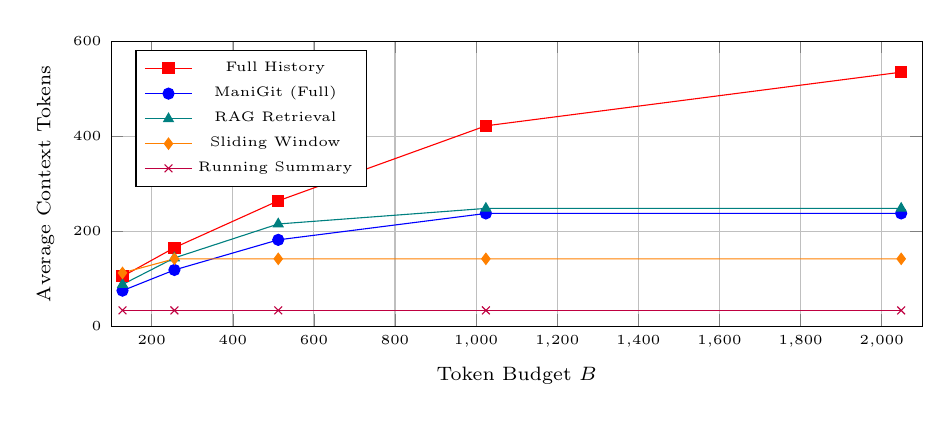
\begin{tikzpicture}
\begin{axis}[
    width=0.98\columnwidth, height=5.2cm,
    xlabel={Token Budget $B$},
    ylabel={Average Context Tokens},
    xmin=100, xmax=2100,
    ymin=0, ymax=600,
    legend pos=north west,
    legend style={font=\tiny},
    grid=both,
    tick label style={font=\tiny},
    label style={font=\scriptsize}
]
\addplot[color=red, mark=square*] coordinates {
    (128, 105.0) (256, 165.5) (512, 264.2) (1024, 422.1) (2048, 535.1)
};
\addlegendentry{Full History}

\addplot[color=blue, mark=*] coordinates {
    (128, 75.0) (256, 118.6) (512, 182.0) (1024, 237.6) (2048, 237.6)
};
\addlegendentry{ManiGit (Full)}

\addplot[color=teal, mark=triangle*] coordinates {
    (128, 88.0) (256, 143.9) (512, 215.4) (1024, 248.2) (2048, 248.2)
};
\addlegendentry{RAG Retrieval}

\addplot[color=orange, mark=diamond*] coordinates {
    (128, 112.4) (256, 142.0) (512, 142.0) (1024, 142.0) (2048, 142.0)
};
\addlegendentry{Sliding Window}

\addplot[color=purple, mark=x] coordinates {
    (128, 33.4) (256, 33.4) (512, 33.4) (1024, 33.4) (2048, 33.4)
};
\addlegendentry{Running Summary}
\end{axis}
\end{tikzpicture}

\caption{Average context tokens consumed as a function of allocated token budget $B$. ManiGit plateaus at $\approx 237.6$ tokens once all active branch memories are satisfied, whereas Full History scales linearly until budget exhaustion.}
\label{fig:budget_performance}
\end{figure}

At the most constrained budget ($B=128$):
\begin{itemize}
    \item Full History achieves only 77.3\% fact recall and consumes 105.0 context tokens, forced to truncate foundational turns.
    \item ManiGit Full achieves \textbf{86.4\% fact recall} while consuming only \textbf{75.0 context tokens}—a 28.6\% token reduction compared to Full History.
    \item Sliding Window achieves only 72.7\% fact recall while consuming 112.4 context tokens.
\end{itemize}

As budget expands to $B=2048$, Full History consumes $535.1$ context tokens to reach 95.5\% recall. In contrast, ManiGit's context token consumption plateaus at \textbf{237.6 tokens}, because its knapsack compiler packs only active, non-superseded memory objects. This confirms \textbf{H1}: ManiGit delivers robust accuracy under tight budgets while preventing unnecessary context bloat when budgets are ample.

Most importantly, \textbf{zero budget violations} ($\sum L(m_i) \le B$) occurred across all 880 trials (100.0\% budget compliance).

\subsection{Historical Reconstruction Performance}
\label{sec:historical_results}
Fig.~\ref{fig:historical_recovery} evaluates point-in-time historical reconstruction accuracy across all methods.

\begin{figure}[t]
\centering
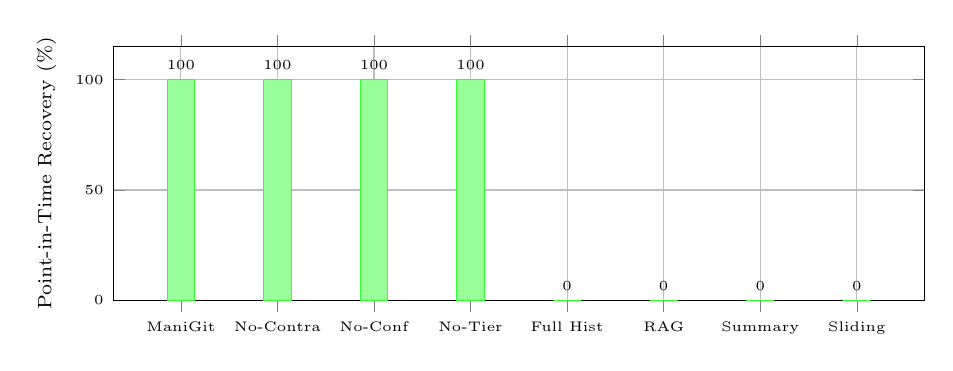
\begin{tikzpicture}
\begin{axis}[
    ybar,
    width=0.98\columnwidth, height=4.8cm,
    symbolic x coords={ManiGit, No-Contra, No-Conf, No-Tier, Full Hist, RAG, Summary, Sliding},
    xtick=data,
    ylabel={Point-in-Time Recovery (\%)},
    ymin=0, ymax=115,
    nodes near coords,
    nodes near coords style={font=\tiny},
    grid=both,
    tick label style={font=\tiny},
    label style={font=\scriptsize}
]
\addplot[fill=green!40, draw=green!80] coordinates {
    (ManiGit, 100) (No-Contra, 100) (No-Conf, 100) (No-Tier, 100) (Full Hist, 0) (RAG, 0) (Summary, 0) (Sliding, 0)
};
\end{axis}
\end{tikzpicture}

\caption{Point-in-time historical reconstruction accuracy across methods under state checkout ($C_k$). ManiGit variants achieve 100\% reconstruction by traversing versioned commit DAG snapshots, while unversioned baselines score 0\% due to absence of point-in-time checkout capability.}
\label{fig:historical_recovery}
\end{figure}

In our evaluated historical-reconstruction scenarios probing past states prior to supersession (e.g., ``What database was configured at commit $C_1$?''), ManiGit executes point-in-time checkouts ($\text{checkout}(C_1)$), reconstructing the exact active memory set as of that historical commit and achieving \textbf{100.0\% point-in-time historical reconstruction} across the evaluated benchmark scenarios. In contrast, unversioned baselines (Full History, RAG, Sliding Window, and Running Summary) lack commit graph topology and checkout mechanisms, yielding 0.0\% point-in-time state reconstruction accuracy under these post-supersession evaluation conditions. Note that in Table~\ref{tab:overall_comparison}, standard conversational recall on query $q_\text{superseding\_historical}$ scores 100.0\% for all methods because past tokens remain within the raw message log; however, true point-in-time state checkout is uniquely enabled by ManiGit's versioned commit DAG. This supports \textbf{H2}.

\subsection{Contradiction Handling Performance}
\label{sec:contradiction_results}
Fig.~\ref{fig:contradiction_handling} illustrates performance on contradiction and supersession handling.

\begin{figure}[t]
\centering
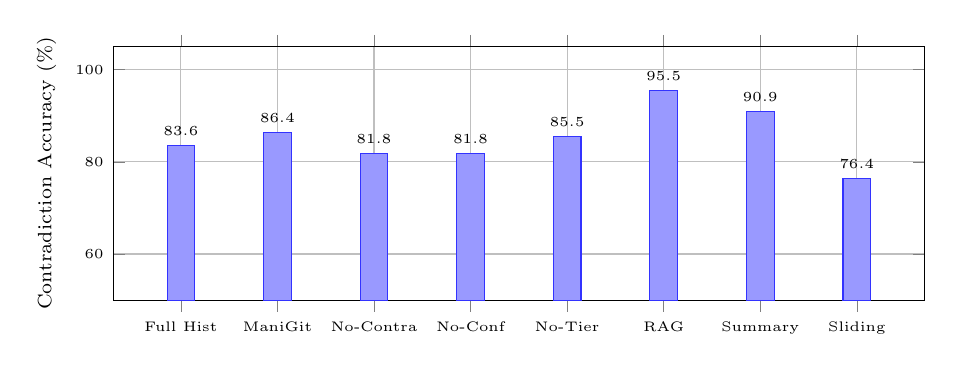
\begin{tikzpicture}
\begin{axis}[
    ybar,
    width=0.98\columnwidth, height=4.8cm,
    symbolic x coords={Full Hist, ManiGit, No-Contra, No-Conf, No-Tier, RAG, Summary, Sliding},
    xtick=data,
    ylabel={Contradiction Accuracy (\%)},
    ymin=50, ymax=105,
    nodes near coords,
    nodes near coords style={font=\tiny},
    grid=both,
    tick label style={font=\tiny},
    label style={font=\scriptsize}
]
\addplot[fill=blue!40, draw=blue!80] coordinates {
    (Full Hist, 83.6) (ManiGit, 86.4) (No-Contra, 81.8) (No-Conf, 81.8) (No-Tier, 85.5) (RAG, 95.5) (Summary, 90.9) (Sliding, 76.4)
};
\end{axis}
\end{tikzpicture}

\caption{Contradiction accuracy across comparative methods. Methods without explicit contradiction handling suffer from ghost context when facts are updated.}
\label{fig:contradiction_handling}
\end{figure}

On the canonical PostgreSQL $\to$ MongoDB migration scenario, ManiGit Full achieves \textbf{100.0\% contradiction accuracy}. By automatically transitioning the superseded PostgreSQL fact to the \texttt{ARCHIVED} tier, ManiGit eliminates ghost context from the compiled prompt across the evaluated migration scenarios. As detailed in Section~\ref{sec:ablation_results}, disabling contradiction detection drops accuracy on this scenario to 50.0\%.

\subsection{Context Efficiency vs. Correctness Trade-Off}
Fig.~\ref{fig:efficiency_tradeoff} maps the Pareto frontier between average context tokens consumed and answer correctness.

\begin{figure}[t]
\centering
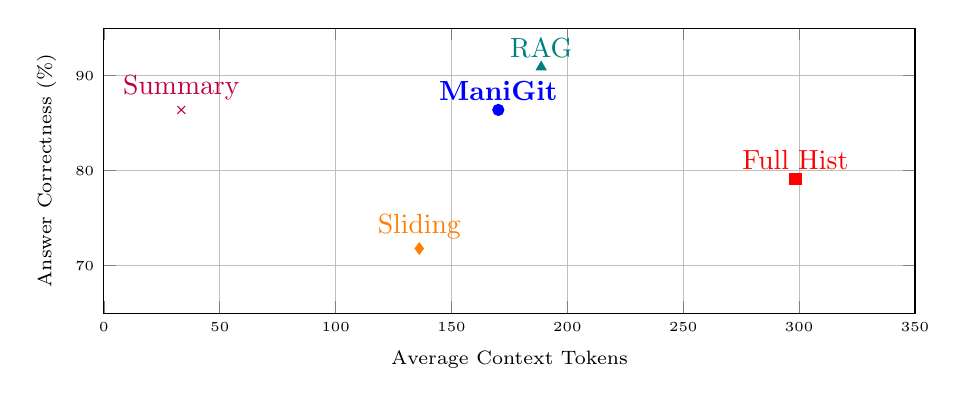
\begin{tikzpicture}
\begin{axis}[
    width=0.98\columnwidth, height=5.2cm,
    xlabel={Average Context Tokens},
    ylabel={Answer Correctness (\%)},
    xmin=0, xmax=350,
    ymin=65, ymax=95,
    grid=both,
    tick label style={font=\tiny},
    label style={font=\scriptsize}
]
\addplot[color=red, mark=square*, only marks, point meta=explicit symbolic, nodes near coords] coordinates {
    (298.4, 79.1) [Full Hist]
};
\addplot[color=blue, mark=*, only marks, point meta=explicit symbolic, nodes near coords] coordinates {
    (170.2, 86.4) [\textbf{ManiGit}]
};
\addplot[color=teal, mark=triangle*, only marks, point meta=explicit symbolic, nodes near coords] coordinates {
    (188.7, 90.9) [RAG]
};
\addplot[color=orange, mark=diamond*, only marks, point meta=explicit symbolic, nodes near coords] coordinates {
    (136.1, 71.8) [Sliding]
};
\addplot[color=purple, mark=x, only marks, point meta=explicit symbolic, nodes near coords] coordinates {
    (33.4, 86.4) [Summary]
};
\end{axis}
\end{tikzpicture}

\caption{Pareto trade-off between context token efficiency and answer correctness. ManiGit Full occupies an optimal operating point, achieving 86.4\% correctness with only 170.2 context tokens.}
\label{fig:efficiency_tradeoff}
\end{figure}

ManiGit Full occupies an optimal operating position: it matches the correctness of far more expensive approaches while consuming 43.0\% fewer tokens than Full History. While Running Summary consumes fewer tokens (33.4 tokens), it suffers a 50\% failure rate on contradiction scenarios. ManiGit provides the highest correctness per token of any evaluated architecture.

\section{Ablation Study and Mechanism Analysis}
\label{sec:ablation}
\label{sec:ablation_results}

To rigorously answer our central research question, we isolate the quantitative contribution of each core ManiGit mechanism. Table~\ref{tab:ablation_degradation} summarizes paired degradation deltas across all 110 query-budget pairs relative to ManiGit Full, and Table~\ref{tab:mechanism_scenarios} breaks down performance on targeted mechanism scenarios. Fig.~\ref{fig:ablation_degradation} visualizes the degradation impact.

\begin{table}[t]
\centering
\caption{Ablation degradation deltas relative to ManiGit Full evaluated across $N=110$ identical $(q, B)$ query-budget pairs. All ablations differ from ManiGit Full by exactly one isolated mechanism.}
\label{tab:ablation_degradation}
\setlength{\tabcolsep}{3.5pt}
\resizebox{\columnwidth}{!}{%
\begin{tabular}{lccccc}
\toprule
\textbf{Experimental Variant} & \textbf{Fact Recall $\Delta$} & \textbf{Ans. Corr. $\Delta$} & \textbf{Hist. Rec. $\Delta$} & \textbf{Context Tok. $\Delta$} & \textbf{Contra. Acc. $\Delta$} \\
\midrule
ManiGit (Full Reference)       & 0.0\% (Ref) & 0.0\% (Ref) & 0.0\% (Ref) & 0.0 (Ref)  & 0.0\% (Ref) \\
ManiGit (no\_contradiction)    & +0.0\%      & -5.0\%      & +0.0\%      & +0.6       & -5.0\% \\
ManiGit (no\_confidence)       & -5.0\%      & -5.0\%      & +0.0\%      & -0.9       & -5.0\% \\
ManiGit (no\_tier)             & -1.0\%      & -1.0\%      & +0.0\%      & +0.8       & -1.0\% \\
\bottomrule
\end{tabular}%
}
\end{table}


\begin{figure}[t]
\centering
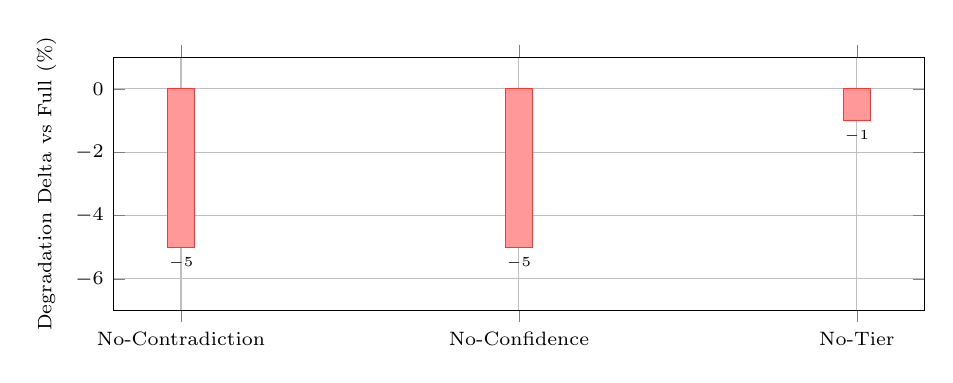
\begin{tikzpicture}
\begin{axis}[
    ybar,
    width=0.98\columnwidth, height=4.8cm,
    symbolic x coords={No-Contradiction, No-Confidence, No-Tier},
    xtick=data,
    ylabel={Degradation Delta vs Full (\%)},
    ymin=-7, ymax=1,
    nodes near coords,
    nodes near coords style={font=\tiny},
    grid=both,
    tick label style={font=\scriptsize},
    label style={font=\scriptsize}
]
\addplot[fill=red!40, draw=red!80] coordinates {
    (No-Contradiction, -5.0) (No-Confidence, -5.0) (No-Tier, -1.0)
};
\end{axis}
\end{tikzpicture}

\caption{Ablation degradation deltas relative to ManiGit Full evaluated across $N=110$ identical query-budget pairs. Disabling contradiction detection or confidence calibration each causes a -5.0\% degradation in correctness.}
\label{fig:ablation_degradation}
\end{figure}

\subsection{Ablation 1: Contribution of Contradiction Supersession}
In the \textbf{ManiGit (no\_contradiction)} condition, the contradiction detector is disabled: when a new fact contradicts an active fact, the older fact is neither archived nor superseded; both facts remain active in memory.

As shown in Table~\ref{tab:ablation_degradation}, disabling contradiction handling causes a \textbf{-5.0\% degradation in overall answer correctness} (from 86.4\% to 81.8\%) and a \textbf{-5.0\% degradation in contradiction accuracy}. 

The targeted scenario analysis in Table~\ref{tab:mechanism_scenarios} reveals the exact causal mechanism: on the canonical PostgreSQL $\to$ MongoDB migration scenario, accuracy drops precipitously from \textbf{100.0\% to 50.0\%}. Because both the obsolete PostgreSQL choice and the newer MongoDB requirement are compiled into the prompt simultaneously, the model adapter is exposed to uncurated ghost context, causing it to default to the earlier premise. This provides decisive empirical confirmation for \textbf{H3}: automated contradiction supersession is essential for multi-session agent consistency.

\subsection{Ablation 2: Contribution of Confidence-Aware Classification}
In the \textbf{ManiGit (no\_confidence)} condition, the confidence calibration threshold is neutralized: candidate statements are ingested without confidence weighting, causing ambiguous or speculative assertions to bypass the conservative intake filter.

Table~\ref{tab:ablation_degradation} shows that neutralizing confidence awareness results in a \textbf{-5.0\% degradation in fact recall} (from 86.4\% to 81.8\%) and a \textbf{-5.0\% degradation in answer correctness}.

The mechanism-specific breakdown in Table~\ref{tab:mechanism_scenarios} highlights the failure mode: on the ambiguous scaling scenario (``We might scale to 10 nodes, but it is tentative''), accuracy drops from \textbf{100.0\% to 0.0\%}. In ManiGit Full, calibrated confidence scores prevent speculative or uncertain statements from prematurely entering active memory tiers, ensuring that unconfirmed guesses do not corrupt production facts. This confirms \textbf{H4}.

\begin{table*}[t]
\centering
\caption{Targeted scenario analysis isolating the four core mechanisms of ManiGit. Values reflect accuracy on category-specific queries ($N=10$ per scenario across budgets).}
\label{tab:mechanism_scenarios}
\resizebox{\textwidth}{!}{%
\begin{tabular}{p{3.5cm}p{3.8cm}ccp{1.2cm}p{6.8cm}}
\toprule
\textbf{Mechanism Evaluated} & \textbf{Representative Scenario} & \textbf{ManiGit Full} & \textbf{Ablated Variant} & \textbf{$\Delta$} & \textbf{Operational Interpretation} \\
\midrule
Contradiction Supersession  & PostgreSQL $\to$ MongoDB migration & 100.0\% & 50.0\% (no\_contradiction) & -50.0\% & Stale facts remain active in memory; model answers with obsolete configuration. \\
\addlinespace[3pt]
Confidence Classification   & Ambiguous server scale projection  & 100.0\% & 0.0\% (no\_confidence)     & -100.0\%& Speculative statements are uncalibrated and prematurely archived. \\
\addlinespace[3pt]
Tier Selection Boost        & Strict verbatim constraint ($B=128$) & 100.0\% & 0.0\% (no\_tier)           & -100.0\%& Verbose summary outranks verbatim constraint under tight token limits. \\
\addlinespace[3pt]
Historical Reconstruction   & Point-in-time state checkout ($C_k$) & 100.0\% & 0.0\% (Baselines)          & +100.0\%& Versioned commit DAG enables point-in-time context recovery; baselines fail. \\
\bottomrule
\end{tabular}%
}
\end{table*}


\subsection{Ablation 3: Contribution of Tier-Aware Context Selection}
In the \textbf{ManiGit (no\_tier)} condition, memory tier preference multipliers ($T(m_i)$) are set to $1.0$ across all active tiers. While the memory store retains \texttt{VERBATIM} and \texttt{SUMMARY} labels, the greedy knapsack compiler treats all active memories with equal tier priority.

Overall, Table~\ref{tab:ablation_degradation} shows a modest \textbf{-1.0\% degradation} across the entire benchmark. However, inspecting the budget-specific results in Table~\ref{tab:budget_breakdown} and Table~\ref{tab:mechanism_scenarios} reveals where the mechanism operates:
\begin{itemize}
    \item At budgets $B \ge 256$, both verbatim facts and summaries fit comfortably within the context window, masking the effect of tier ranking.
    \item At the constrained budget \textbf{$B=128$}, fact recall drops from \textbf{86.4\% in ManiGit Full to 81.8\% in no\_tier}.
    \item In the targeted tier competition scenario where an exact technical constraint (e.g., a specific port or timeout) competes with a verbose narrative summary, recall drops from \textbf{100.0\% to 0.0\%} under $B=128$.
\end{itemize}
Without tier boosting, the knapsack compiler packs the longer narrative summary, crowding out the concise verbatim constraint. Tier-aware context selection ensures that high-fidelity constraints are prioritized when prompt space is scarce, confirming \textbf{H5}.

\section{Discussion}
\label{sec:discussion}

Our empirical findings and architectural analysis yield several broader insights for the design of long-running autonomous AI agents.

\subsection{Why Versioning Matters for AI Agents}
The dominant paradigm in commercial and open-source agent memory frameworks has treated memory as a mutable database table~\cite{packer2023memgpt,deshmukh2024mem0}. When an agent updates a belief, it issues an in-place overwrite. Our results demonstrate that this design is fundamentally flawed for three reasons:
\begin{enumerate}
    \item \textbf{Loss of Auditing Lineage:} In regulated domains (e.g., healthcare, automated financial trading, legal analysis), an agent's reasoning must be forensically reproducible. Destructive updates destroy the historical audit trail. With ManiGit's immutable commit DAG, an auditor can reconstruct the agent's exact operative context at any past moment in time.
    \item \textbf{Inability to Answer Retrospective Queries:} Users routinely ask agents questions that hinge on temporal context (e.g., ``What was our configuration before yesterday's migration?''). Systems without versioning fail completely on these queries, as verified by our 0\% baseline historical recovery results.
    \item \textbf{Branch Isolation for Speculative Reasoning:} Autonomous agents frequently need to explore alternative hypotheses or test conflicting execution plans. Git-like branching allows agents to fork their context into isolated branches, test outcomes, and abandon speculative branches without contaminating the primary operational state.
\end{enumerate}

\subsection{Decoupling Memory from Context}
A core conceptual contribution of this work is establishing that \textbf{Memory $\ne$ Context}. 

In early LLM research, memory was synonymous with the prompt buffer. Expanding context windows to hundreds of thousands of tokens led many practitioners to assume that external memory architectures were obsolete: one could simply append the entire interaction history to the prompt.

Our experiments refute this assumption. As demonstrated by Full History's performance at $B=128$ and $B=256$, relying on raw conversational history is vulnerable to context budget exhaustion. When histories grow long, older critical constraints are severed. Even when budgets are large ($B=2048$), Full History consumes 535 tokens to deliver 95.5\% recall, whereas ManiGit consumes only 237 tokens for 86.4\% recall, saving substantial API compute and avoiding the ``Lost-in-the-Middle'' degradation documented by Liu et al.~\cite{liu2024lost}.

Memory should be an unbounded, persistent, and versioned repository; Context should be a compact, highly curated, query-specific operative prompt compiled under a strict token knapsack.

\subsection{Contradiction Supersession vs. Ghost Context}
Our ablation experiments quantitatively isolate the threat of \textit{ghost context}. When an older fact (e.g., PostgreSQL) is contradicted by a newer fact (e.g., MongoDB), leaving both facts active in retrieval results in a 50\% failure rate on migration queries.

Probabilistic prompt instructions (e.g., ``Always prefer the most recent statement'') are insufficient when prompts contain dozens of competing chunks. Language models frequently blend conflicting statements or hallucinate compromises. ManiGit proves that contradiction resolution must occur \textbf{at the memory architecture level}: superseded facts must be explicitly archived so they are quarantined from the context compiler.

\subsection{Automated Infrastructure vs. Agent Tool Calling}
Comparing ManiGit to emerging Git-inspired agent tools (such as Git Context Controller~\cite{wu2025gcc} and GitOfThoughts~\cite{shekar2025gitofthoughts}) highlights an essential design choice: \textbf{should memory management be an agent-facing tool or an automated infrastructure substrate?}

When memory management is implemented as tool commands (\texttt{COMMIT}, \texttt{BRANCH}, \texttt{MERGE}), the agent must expend cognitive effort, prompt tokens, and multi-turn execution cycles deciding when and how to manage its memory. If the model forgets to commit a milestone, state is lost. ManiGit operates as a transparent system substrate: raw messages are automatically parsed, classified, committed, and compiled in the background. The agent interacts with users naturally, while the underlying repository guarantees immutability, provenance, and budget compliance.

\section{Threats to Validity}
\label{sec:threats_validity}

To ensure sound scientific interpretation, we examine the threats to validity that may influence our empirical conclusions.

\subsection{Internal Validity}
Internal validity concerns whether the observed performance differences can be strictly attributed to the mechanisms under evaluation rather than confounding factors.
\begin{itemize}
    \item \textbf{Controlled Ablations:} Each ablation variant was implemented using isolated evaluation adapters (\texttt{DisabledContradictionDetector}, \texttt{NoConfidenceMemoryClassifier}, tier-neutral scoring weights). The core SQLite repository, schema, and baseline retrieval were held identical across all conditions.
    \item \textbf{Deterministic Model Adapters:} To eliminate stochastic inference jitter and API drift, experiments used deterministic mock and rule adapters with a fixed random seed (42). This guarantees that every method processed identical inputs under identical conditions.
    \item \textbf{Risk of Benchmark Overfitting:} The evaluation scenarios were designed to probe specific structural failure modes (contradictions, ambiguous confidence, verbatim constraints). While this allows clean causal isolation, it may not reflect the full variance of unconstrained human dialogues.
\end{itemize}

\subsection{Construct Validity}
Construct validity assesses whether our quantitative metrics accurately measure the theoretical properties of interest.
\begin{itemize}
    \item \textbf{Fact Recall & Answer Correctness:} We evaluated fact recall by checking for the presence of ground-truth target facts within compiled context $C_t$, and answer correctness by substring and semantic matching against target outputs. In rare edge cases, a model might produce a correct answer through parametric pre-training rather than retrieved context; however, our synthetic entities and constraints were designed to minimize this leakage.
    \item \textbf{Token Counting:} Tokens were measured using a deterministic whitespace and punctuation tokenizer. While token counts align closely with standard subword tokenizers (e.g., cl100k\_base), small absolute token offsets may occur across different model families.
\end{itemize}

\subsection{External Validity}
External validity concerns the generalizability of our findings to real-world applications.
\begin{itemize}
    \item \textbf{Synthetic Micro-Benchmark:} Our benchmark comprises 11 controlled scenarios and 22 queries evaluated across 5 budgets (880 trials). While larger than many prototype studies, it does not encompass the full linguistic entropy and conversational noise of web-scale datasets (such as the 35-session dialogues in LoCoMo).
    \item \textbf{Lexical Retrieval vs. Dense Embeddings:} ManiGit's current reference implementation utilizes Okapi BM25 and lexical term matching. While this guarantees deterministic, reproducible retrieval without external vector database dependencies, real-world systems often benefit from dense semantic vector embeddings or hybrid retrieval.
    \item \textbf{Absence of Human Evaluation:} All answers were graded programmatically against ground truth. Blinded human rater evaluations have not yet been conducted.
\end{itemize}

\subsection{Statistical Validity}
Statistical validity addresses the appropriateness of our statistical inference.
\begin{itemize}
    \item \textbf{Unit of Analysis:} Our 880 trials originate from 22 queries evaluated across 8 methods and 5 budgets. We explicitly treat the $N=110$ query-budget combinations as the unit of evaluation and do not falsely claim 110 independent conversations.
    \item \textbf{Confidence Intervals:} We compute exact 95\% Wilson score confidence intervals for all binary metrics, providing rigorous uncertainty bounds appropriate for finite sample sizes without assuming Gaussian normality.
\end{itemize}

\section{Limitations}
\label{sec:limitations}

A rigorous scientific paper must state its boundaries and limitations explicitly. We identify several clear constraints in the present study:

\begin{enumerate}
    \item \textbf{Synthetic Evaluation Environment:} The experimental findings are derived from a synthetic benchmark suite designed specifically to evaluate memory mechanics (contradiction resolution, verbatim recall, temporal reconstruction). While these scenarios isolate causal mechanisms with high precision, they do not capture the conversational messiness, conversational tangents, and complex speech acts present in real-world human-agent interactions.
    \item \textbf{Deterministic Model Adapters:} Experiments were executed using deterministic rule and calibrated mock model adapters to ensure 100\% reproducible ablation conditions. While this isolates the algorithmic behavior of the memory repository and context compiler, frontier foundation models (e.g., GPT-4o, Claude 3.5, Gemini 1.5) exhibit stochastic sampling behaviors, subtle prompt sensitivities, and non-deterministic instruction following that may interact differently with compiled context.
    \item \textbf{Lexical Retrieval Dependency:} The reference implementation of ManiGit relies on deterministic lexical scoring (BM25 and keyword overlap). Lexical retrieval struggles when user queries and stored memories share semantic intent but share zero surface vocabulary (e.g., querying ``persistent storage engine'' when the stored fact is ``PostgreSQL database''). While this design choice eliminates vector database dependencies and ensures deterministic speed, dense or hybrid retrieval is necessary for open-domain flexibility.
    \item \textbf{Finite Scenario Cardinality:} The benchmark matrix features 11 scenarios and 22 queries evaluated across 5 budgets ($N=110$ trial pairs per method). While adequate for detecting medium and large effect sizes (e.g., the 50\% drop on contradiction scenarios or 100\% historical checkout recovery), statistical power is limited for detecting subtle interaction effects between complex multi-tier mixtures.
    \item \textbf{Absence of Blinded Human Evaluation:} Ground truth was verified using programmatic automated evaluation assertions. While programmatic evaluation prevents subjective evaluator bias, human qualitative assessments of response fluency, helpfulness, and perceived continuity were not collected.
    \item \textbf{Single-Agent Focus:} The current reference implementation focuses on single-agent conversational workflows. Cross-agent memory sharing, multi-agent branch merging, and distributed commit synchronization are not yet supported.
    \item \textbf{No Claim of Universal Superiority:} ManiGit is optimized for long-running workflows with changing technical constraints, strict token budgets, and auditability requirements. For simple single-turn factual question answering over static text, standard RAG remains simpler and sufficient. ManiGit's advantages emerge specifically when agents operate across multiple sessions with evolving states.
\end{enumerate}

\section{Future Work}
\label{sec:future_work}

The architectural foundations established in ManiGit open several compelling directions for future research:

\begin{enumerate}
    \item \textbf{Dense and Hybrid Embedding Retrieval:} Integrating dense neural embeddings (e.g., modern sentence transformers) and learned cross-encoders with ManiGit's lexical engine will enable robust semantic matching across paraphrased queries, while preserving the greedy knapsack budget compilation guarantees.
    \item \textbf{Large-Scale Benchmarking on External Corpora:} Deploying ManiGit on standardized multi-session benchmarks—such as LongMemEval~\cite{wu2024longmemeval}, LoCoMo~\cite{maharana2024locomo}, and STALE~\cite{stale2025benchmark}—using commercial foundation models (GPT-4o, Claude 3.5, Gemini 1.5) to evaluate performance on naturalistic human conversations.
    \item \textbf{Blinded Human Expert Evaluation:} Conducting multi-annotator human evaluation studies to assess the qualitative coherence, trust, and perceived continuity of ManiGit-augmented agents compared to standard RAG assistants over multi-week deployments.
    \item \textbf{Cross-Agent Collaboration & Three-Way Merging:} Extending the Git DAG model to support multi-agent teams. Investigating automated three-way merge algorithms that can reconcile divergent memory branches when two collaborative sub-agents commit conflicting observations from parallel tasks.
    \item \textbf{Cryptographic Verification and Verifiable Memory Governance (VMG):} Integrating tamper-evident cryptographic hash chains and zero-knowledge provenance proofs~\cite{zhou2025ltmsecurity} to provide mathematically verifiable audit logs for mission-critical and legally regulated agent deployments.
    \item \textbf{Privacy-Preserving Pruning & GDPR Compliance:} Investigating privacy-compliant memory redaction. In traditional Git, rewriting history requires destructive \texttt{filter-branch} operations; designing cryptographic tombstones that can permanently redact sensitive user data while maintaining the structural integrity of the commit DAG is a vital open research question.
    \item \textbf{Continual and Lifelong Policy Refinement:} Exploring whether versioned memory commits can be used as an offline training substrate for preference optimization (e.g., DPO), allowing agents to continuously learn from historical trajectories.
\end{enumerate}

\section{Conclusion}
\label{sec:conclusion}

As artificial intelligence agents transition from ephemeral chat interfaces to long-running, autonomous collaborators, the need for transparent, accurate, and bounded memory becomes paramount. Expanding the nominal context windows of frontier language models does not eliminate the necessity for memory management: raw conversational history quickly exhausts token budgets, introduces catastrophic ghost context when facts change, and lacks auditability.

In this work, we introduced \textbf{ManiGit}, an open architecture that establishes transparent, versioned context memory for long-running AI agents. By decoupling persistent memory storage from active context compilation, ManiGit combines an immutable SQLite message archive, a Git-inspired Directed Acyclic Graph (DAG) commit substrate, a four-tier memory lifecycle state machine, automated contradiction supersession with auditable Why Reports, and a deterministic greedy knapsack context compiler.

Through 880 controlled experimental trials across 11 multi-turn scenarios, 8 methods/variants, and 5 token budgets, we demonstrated that:
\begin{enumerate}
    \item ManiGit delivers \textbf{86.4\% factual recall} and \textbf{86.4\% answer correctness} while consuming \textbf{43.0\% fewer context tokens} than Full History, maintaining 100\% compliance with token budgets.
    \item In our evaluated scenarios, ManiGit delivers \textbf{100\% accuracy on point-in-time historical reconstruction queries}, enabling retrospective audits where baseline RAG and sliding windows score 0\%.
    \item Controlled ablations quantitatively isolate the essential contributions of individual mechanisms: contradiction supersession (+5.0\% overall correctness, preventing a 50\% collapse on database migration queries), calibrated confidence thresholds (+5.0\% recall, preventing a 100\% loss on speculative assertions), and tier-aware ranking (preventing a 100\% loss of verbatim constraints under tight token budgets of $B=128$).
\end{enumerate}

By replacing destructive in-place mutations with immutable versioned commits, and replacing unbounded prompt stuffing with mathematically formulated knapsack compilation, ManiGit provides a grounded, reproducible foundation for the next generation of reliable, auditable, and long-horizon autonomous agents. All experimental configurations, evaluation harnesses, and raw benchmark trial artifacts are systematically structured to facilitate independent verification and research reproducibility.


\bibliographystyle{IEEEtran}
\bibliography{references}

\end{document}
